\documentclass[9pt]{beamer}
\usetheme{Madrid}
\setbeamercovered{invisible}
\setbeamertemplate{navigation symbols}{}


\usepackage{graphicx}
\usepackage{tabularx}
\usepackage{subfig}





\title[Oral presentation]{Development and accuracy evaluation of Coded phase-shift 3D scanner}
\author{Pranav Kant Gaur,D.M.Sarode,S.K.Bose}
\institute[Computer Division, Bhabha Atomic Research Centre]
{
Graphics and Visualization Section\\
Computer Division\\
Bhabha Atomic Research Centre \\
\medskip
{\emph{pranav@barc.gov.in}}
}
\date{23/Aug/2013}


\begin{document}

%%%%%%%%%%%%%%%%%%%%%%%%%%%%%%%%%%%%%%%%%%%%%%%%%%%%%%%%%%%%%%%%%%%%%%%%%%%%%SLIDE starts%%%%%%%%%%%%%%%%%%%%%%%%%%%%%%%%%%%%%
\begin{frame}
\titlepage
\end{frame}
%%%%%%%%%%%%%%%%%%%%%%%%%%%%%%%%%%%%%%%%%%%%%%%%%%%%%%%%%%%%%%%%%%%%%%%%%%%%%SLIDE ENDS%%%%%%%%%%%%%%%%%%%%%%%%%%%%%%%%%%%%%%%



%%%%%%%%%%%%%%%%%%%%%%%%%%%%%%%%%%%%%%%%%%%%%%%%%%%%%%%%%%%%%%%%%%%%%%%%%%%%%SLIDE starts%%%%%%%%%%%%%%%%%%%%%%%%%%%%%%%%%%%%%
\begin{frame}
\frametitle{Agenda}
\begin{enumerate}
\item Introduction
\item Approach used
\item 3D scanner system:Overview
\item Developement
\item Accuracy evaluation
\item Conclusions
\end{enumerate}
\end{frame}
%%%%%%%%%%%%%%%%%%%%%%%%%%%%%%%%%%%%%%%%%%%%%%%%%%%%%%%%%%%%%%%%%%%%%%%%%%%%%SLIDE ENDS%%%%%%%%%%%%%%%%%%%%%%%%%%%%%%%%%%%%%%%


%%%%%%%%%%%%%%%%%%%%%%%%%%%%%%%%%%%%%%%%%%%%%%%%%%%%%%%%%%%%%%%%%%%%%%%%%%%%%SLIDE starts%%%%%%%%%%%%%%%%%%%%%%%%%%%%%%%%%%%%%
\begin{frame}
\frametitle{Introduction}
\begin{enumerate}
\item What?
\begin{enumerate}
\item 3D scanner
\begin{enumerate}
  \item Digital reconstruction of real world scene.
\end{enumerate}
\end{enumerate}

\item Why?
\begin{enumerate}
\item Applications
\begin{enumerate}
   \item Medical: Dental model reconstruction for teeth implantation
   \item Scientific analysis: Study of dynamics for example, C.F.D, machine component dynamics etc.
   \item Biometric security: 3D face authentication, thumb pattern authentication
   \item Entertainment : XBOX Kinect etc.
\end{enumerate}
\end{enumerate}

\item How?
\begin{enumerate}
\item Key problems
\begin{enumerate}
   \item Stereo correspondence: At least 2 views required
   \item System calibration: Mapping measurement units of optical elements to physical units(mm,feet etc.) 
   \item Triangulation: Compute 3D coordinates given system calibration and stereo correspondence
\end{enumerate}
\end{enumerate}
\end{enumerate}
\end{frame}
%%%%%%%%%%%%%%%%%%%%%%%%%%%%%%%%%%%%%%%%%%%%%%%%%%%%%%%%%%%%%%%%%%%%%%%%%%%%%SLIDE ENDS%%%%%%%%%%%%%%%%%%%%%%%%%%%%%%%%%%%%%%%

%%%%%%%%%%%%%%%%%%%%%%%%%%%%%%%%%%%%%%%%%%%%%%%%%%%%%%%%%%%%%%%%%%%%%%%%%%%%%SLIDE starts%%%%%%%%%%%%%%%%%%%%%%%%%%%%%%%%%%%%%
\begin{frame}
\frametitle{Approach used}
\begin{enumerate}
\item Stereo correspondence:
\begin{enumerate}
\item Coded phase shift approach
\begin{figure}[ht]
\begin{tabularx}{\linewidth}{@{}cXX@{}}
\begin{tabular}{c c}
\hspace{1cm}\subfloat[Phase shift approach]{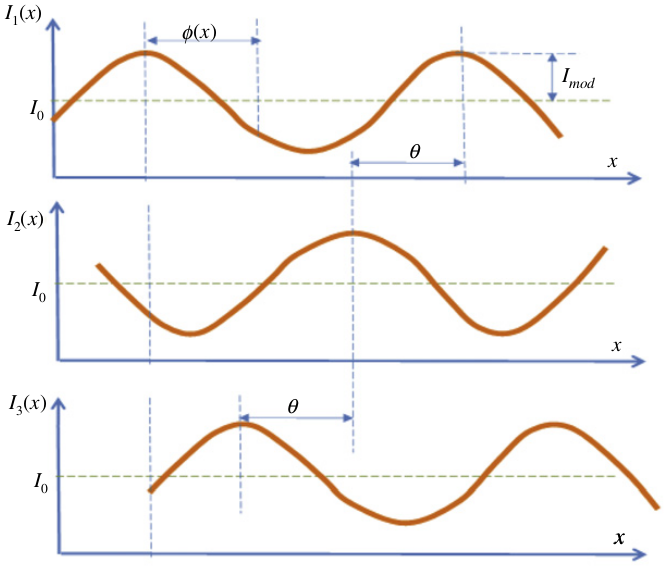
\includegraphics[width=3.5cm,height=3cm]{dependencies/img_source/phase_shifted.jpg}} &
\subfloat[Binary coded approach]{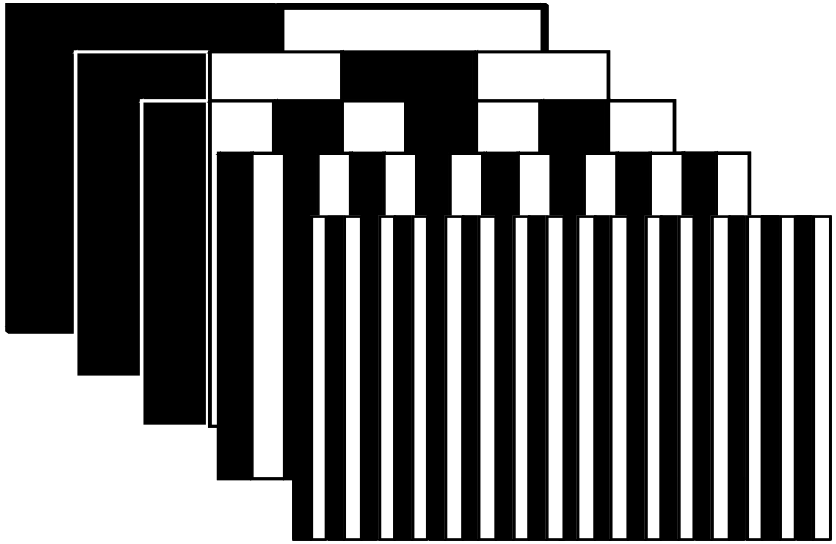
\includegraphics[width=3.5cm,height=3cm]{dependencies/img_source/binary_codes.jpg}}\\    
\end{tabular}
\end{tabularx}
\caption{Solving stereo correspondence} % to be fixed (why needed??) 
\end{figure}
\end{enumerate}
\end{enumerate}
\begin{enumerate}
\item System calibration
\begin{enumerate}
\item OpenCV camera calibration and VPCLib projector calibration algorithm used.
\end{enumerate}
\end{enumerate}
\begin{enumerate}
\item Triangulation
\begin{enumerate}
\item Camera and projector model equations are solved for corresponding camera and projector pixels.
\end{enumerate}
\end{enumerate}

\end{frame}
%%%%%%%%%%%%%%%%%%%%%%%%%%%%%%%%%%%%%%%%%%%%%%%%%%%%%%%%%%%%%%%%%%%%%%%%%%%%%SLIDE ENDS%%%%%%%%%%%%%%%%%%%%%%%%%%%%%%%%%%%%%%%





%%%%%%%%%%%%%%%%%%%%%%%%%%%%%%%%%%%%%%%%%%%%%%%%%%%%%%%%%%%%%%%%%%%%%%%%%%%%%SLIDE starts%%%%%%%%%%%%%%%%%%%%%%%%%%%%%%%%%%%%%
\begin{frame}
\frametitle{3D scanner system:Overview}
\begin{figure}[ht]
\begin{tabularx}{\linewidth}{@{}cXX@{}}
\begin{tabular}{c c}
\vspace{6cm}\subfloat[System setup]{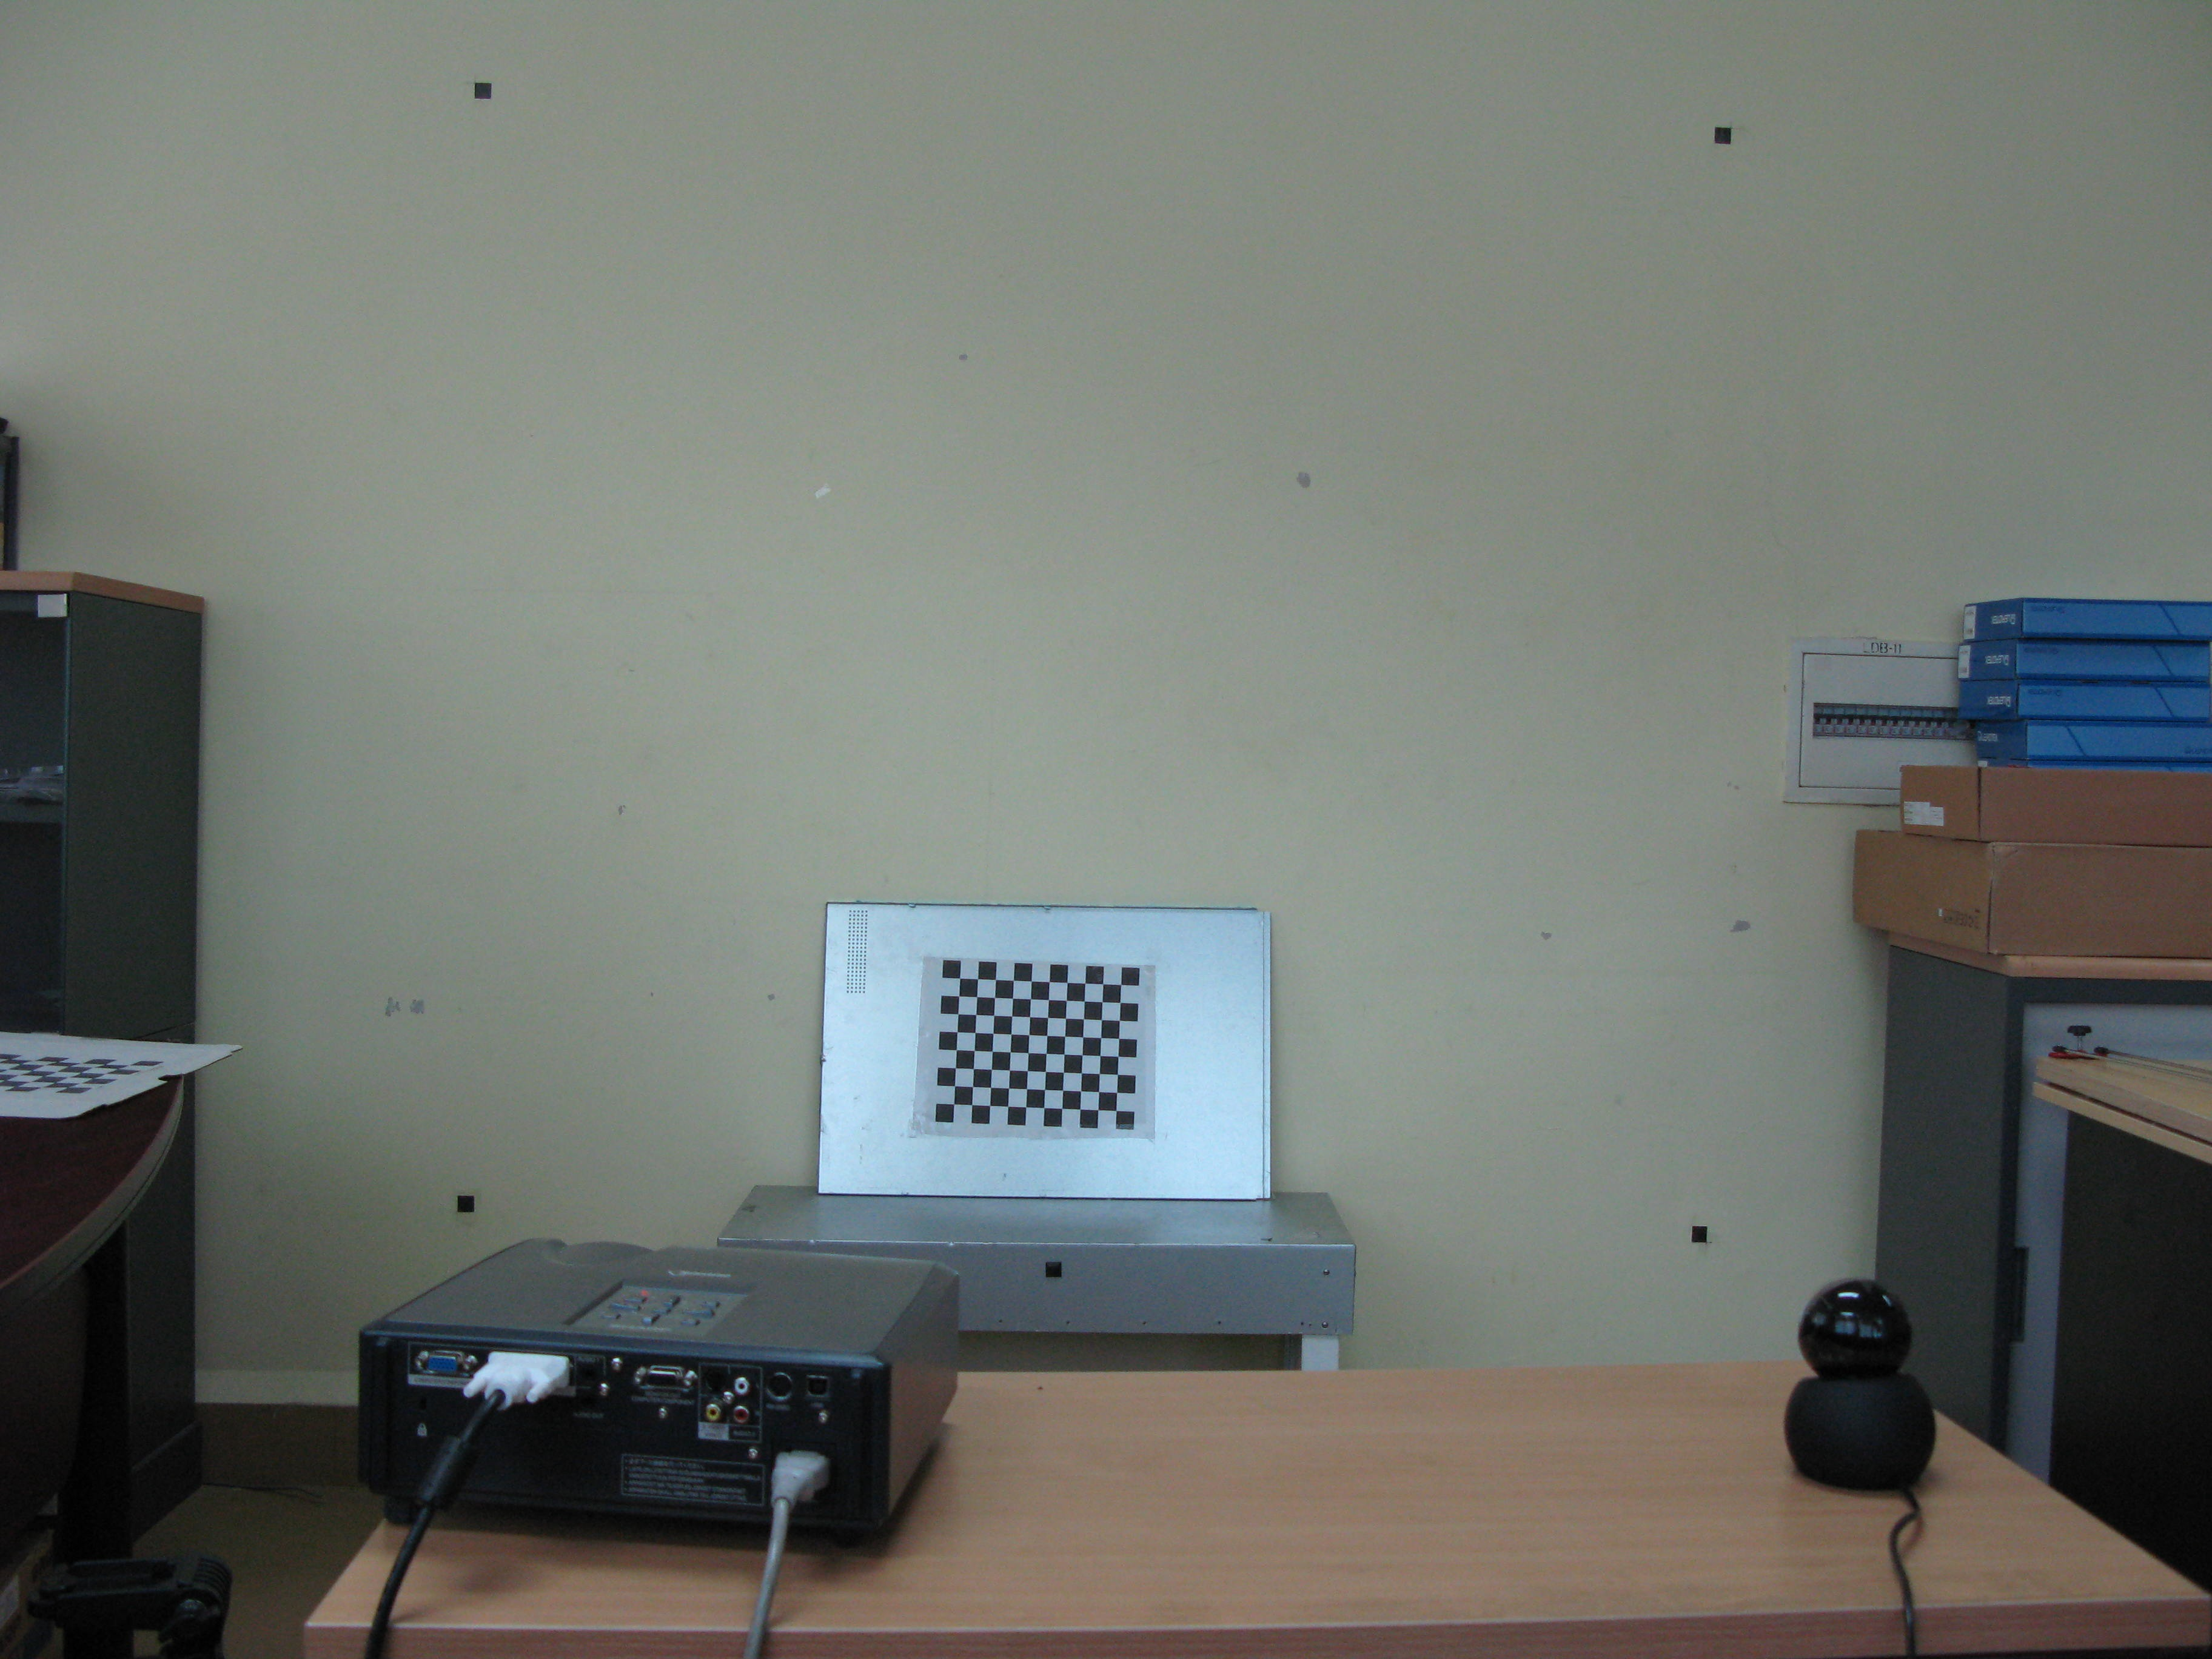
\includegraphics[width=4cm,height=4cm]{dependencies/img_source/system_setup.jpg}} &
\subfloat[Software architecture]{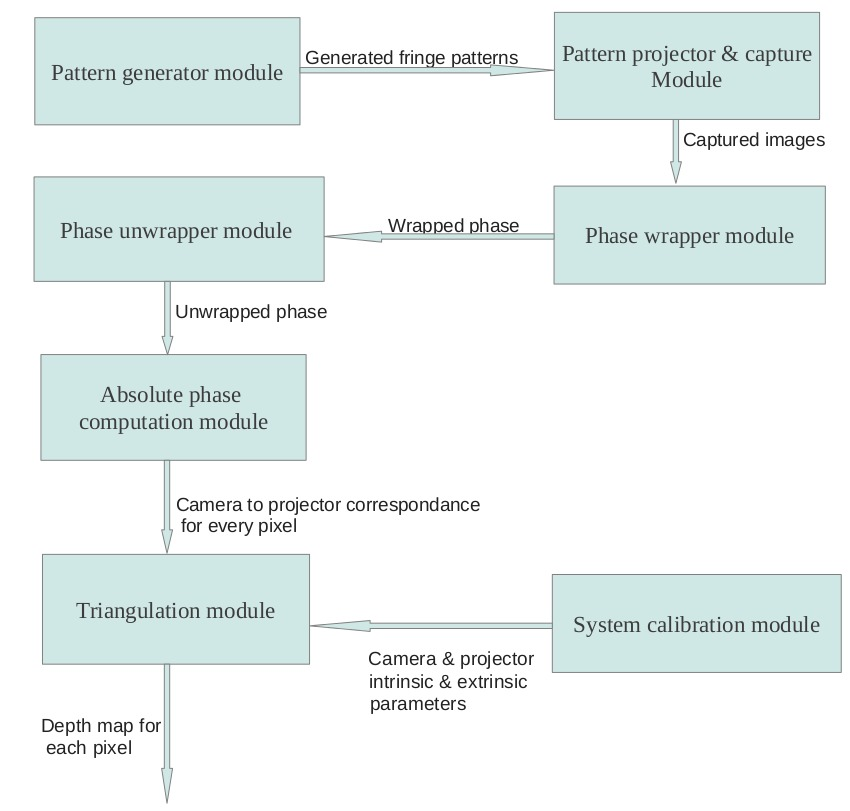
\includegraphics[width=7cm,height=7.5cm]{dependencies/img_source/system_layout.jpg}}\\    
\end{tabular}
\end{tabularx}
\caption{hi there} % to be fixed (why needed??) 
\end{figure}

\end{frame}
%%%%%%%%%%%%%%%%%%%%%%%%%%%%%%%%%%%%%%%%%%%%%%%%%%%%%%%%%%%%%%%%%%%%%%%%%%%%%SLIDE ENDS%%%%%%%%%%%%%%%%%%%%%%%%%%%%%%%%%%%%%%%


%%%%%%%%%%%%%%%%%%%%%%%%%%%%%%%%%%%%%%%%%%%%%%%%%%%%%%%%%%%%%%%%%%%%%%%%%%%%%SLIDE starts%%%%%%%%%%%%%%%%%%%%%%%%%%%%%%%%%%%%%
\begin{frame}
\frametitle{System calibration}
\begin{figure}[ht]
\begin{tabularx}{\linewidth}{@{}cXX@{}}
\begin{tabular}{c c c}
\hspace{-0.5cm}\subfloat[Camera calibration]{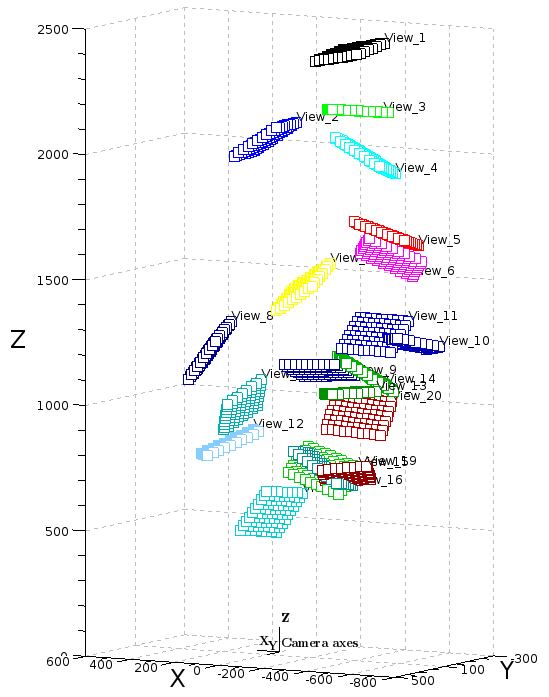
\includegraphics[width=3.5cm,height=6cm]{dependencies/img_source/cam_calib_plot_better.png}} &
\subfloat[Projector calibration]{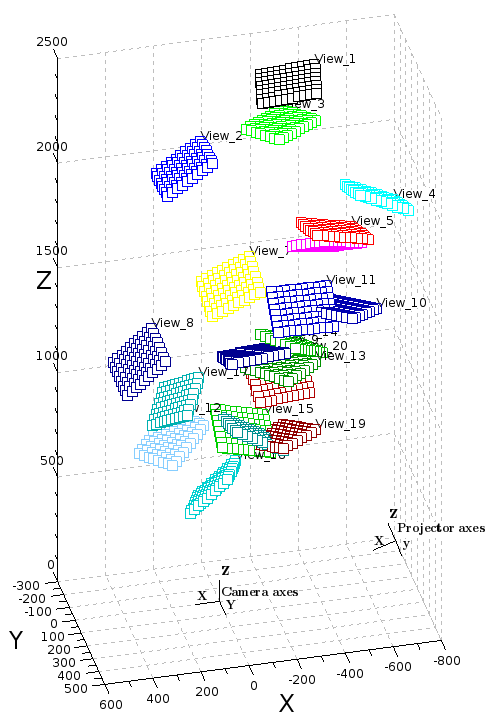
\includegraphics[width=3.5cm,height=6cm]{dependencies/img_source/proj_calib_plot_better.png}} &
\subfloat[Extrinsic calibration]{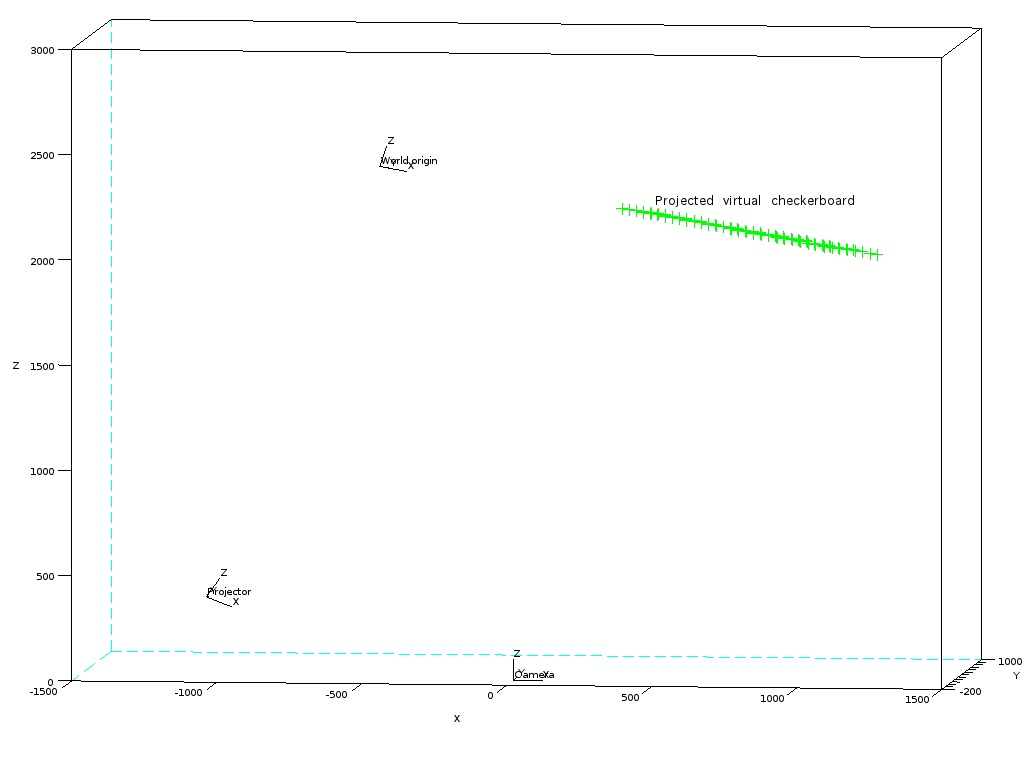
\includegraphics[width=5cm,height=6cm]{dependencies/img_source/system_plot_edit.jpg}} \\
\end{tabular}
\end{tabularx}
\end{figure}
\end{frame}
%%%%%%%%%%%%%%%%%%%%%%%%%%%%%%%%%%%%%%%%%%%%%%%%%%%%%%%%%%%%%%%%%%%%%%%%%%%%%SLIDE ENDS%%%%%%%%%%%%%%%%%%%%%%%%%%%%%%%%%%%%%%%


%%%%%%%%%%%%%%%%%%%%%%%%%%%%%%%%%%%%%%%%%%%%%%%%%%%%%%%%%%%%%%%%%%%%%%%%%%%%%SLIDE starts%%%%%%%%%%%%%%%%%%%%%%%%%%%%%%%%%%%%%
\begin{frame}
\frametitle{Pattern generation}
Model for phase shifted sinusoidal patterns:
\begin{equation}
\begin{aligned}
& P_1^v=A_v+B_v*cos(\theta_v-\alpha) \\
& P_2^v=A_v+B_v*cos(\theta_v) \\
& P_3^v=A_v+B_v*cos(\theta_v+\alpha) \\
\end{aligned}
\end{equation}
where $\theta_v=2\pi\frac{x}{fringe\ width}$\newline
\newline Model for binary coded patterns:
\begin{equation}
N_{v}^{codes}=\frac{W_{projector}}{w_{fringe}} 
\end{equation}
\begin{equation}
N_{v}^{patterns}=\log_2(N_v^{codes})
\end{equation}
\begin{equation}
Intensity_{(i,j)}=\lfloor i/{(w_{fringe}*2^{pattern\ number})} \rfloor
\end{equation}    

\begin{figure}[ht]
%\def\tabularxcolumn#1{m{#1}}
\begin{tabularx}{\linewidth}{@{}cXX@{}}
\begin{tabular}{c c c c c c}
\subfloat[]{
\includegraphics[width=1.5cm,height=1cm]{dependencies/img_source/phase_ver_1.jpg}} &
\subfloat[]{
\includegraphics[width=1.5cm,height=1cm]{dependencies/img_source/phase_ver_2.jpg}} &
\subfloat[]{
\includegraphics[width=1.5cm,height=1cm]{dependencies/img_source/phase_ver_3.jpg}} &
\subfloat[]{
\includegraphics[width=1.5cm,height=1cm]{dependencies/img_source/binary_ver_1.jpg}} &
\subfloat[]{
\includegraphics[width=1.5cm,height=1cm]{dependencies/img_source/binary_ver_2.jpg}} &
\subfloat[]{
\includegraphics[width=1.5cm,height=1cm]{dependencies/img_source/binary_ver_3.jpg}} \\
\end{tabular}
\end{tabularx}
\caption{Vertical phase-shifted patterns \& binary coded patterns}
\end{figure}
\end{frame}
%%%%%%%%%%%%%%%%%%%%%%%%%%%%%%%%%%%%%%%%%%%%%%%%%%%%%%%%%%%%%%%%%%%%%%%%%%%%%SLIDE ENDS%%%%%%%%%%%%%%%%%%%%%%%%%%%%%%%%%%%%%%%

%%%%%%%%%%%%%%%%%%%%%%%%%%%%%%%%%%%%%%%%%%%%%%%%%%%%%%%%%%%%%%%%%%%%%%%%%%%%%SLIDE starts%%%%%%%%%%%%%%%%%%%%%%%%%%%%%%%%%%%%%
\begin{frame}
\frametitle{Pattern projection and capture}
\vspace{-0.5cm}
\begin{figure}
\centering
\begin{tabularx}{\linewidth}{@{}cXX@{}}
\begin{tabular}{c c c}
\subfloat[]{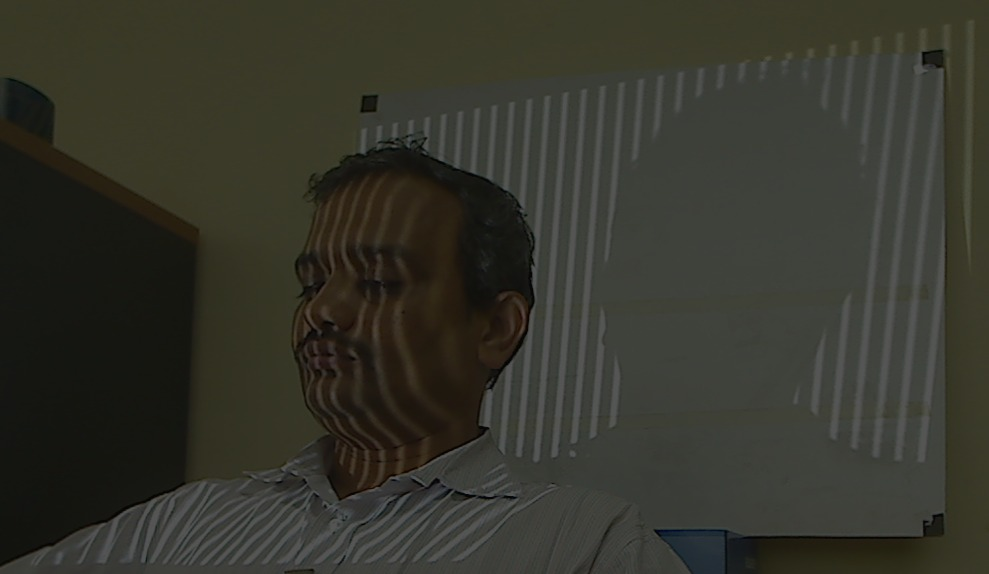
\includegraphics[width=3.5cm,height=3cm]{dependencies/img_source/cap_fringe_v1.jpg}} &
\subfloat[]{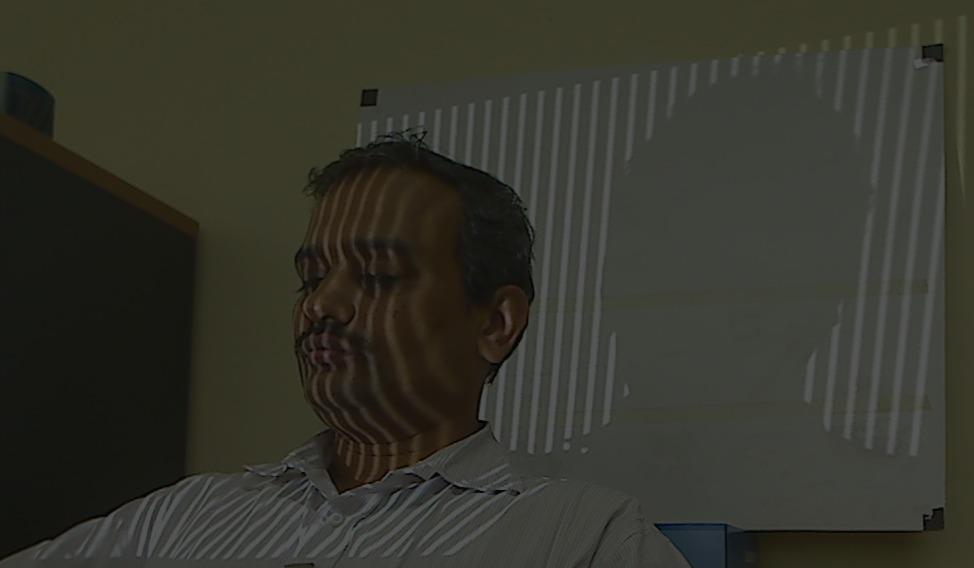
\includegraphics[width=3.5cm,height=3cm]{dependencies/img_source/cap_fringe_v2.jpg}} &
\subfloat[]{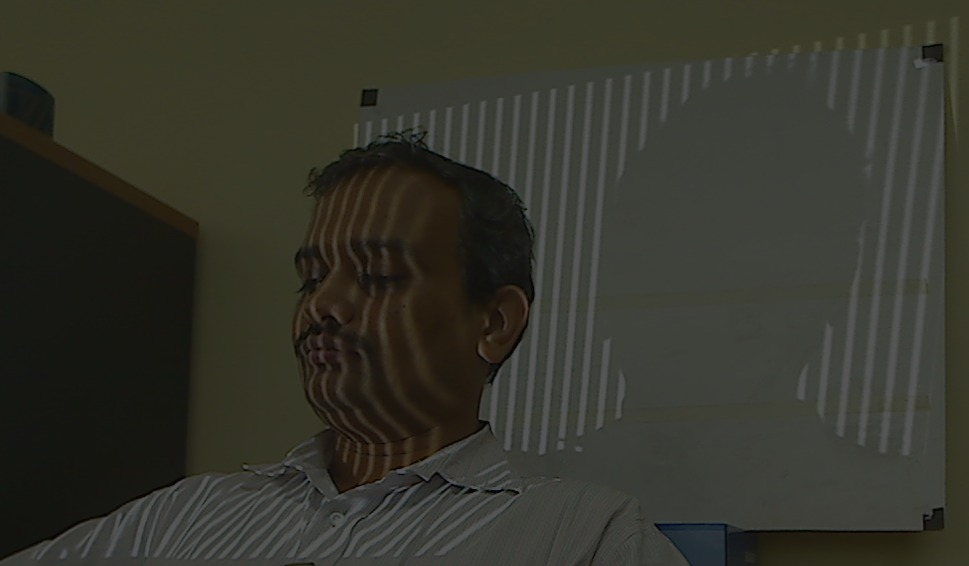
\includegraphics[width=3.5cm,height=3cm]{dependencies/img_source/cap_fringe_v3.jpg}} \\
\end{tabular}
\end{tabularx}
\caption{Captured vertical phase-shifted patterns}
\end{figure}
\vspace{-0.5cm}
\begin{figure}
\centering
\begin{tabularx}{\linewidth}{@{}cXX@{}}
\begin{tabular}{c c c}
\subfloat[]{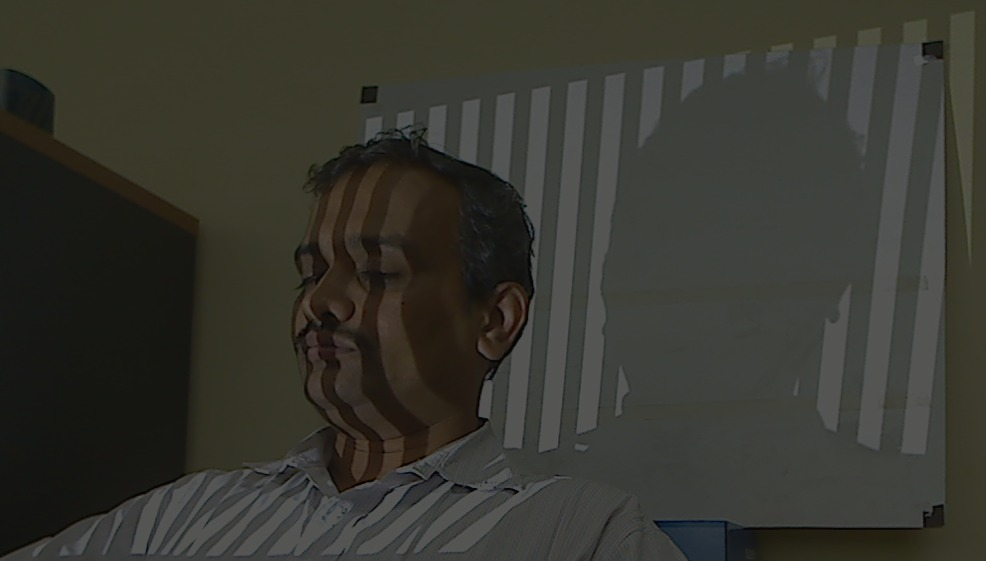
\includegraphics[width=3.5cm,height=3cm]{dependencies/img_source/cap_binary_v1.jpg}} &
\subfloat[]{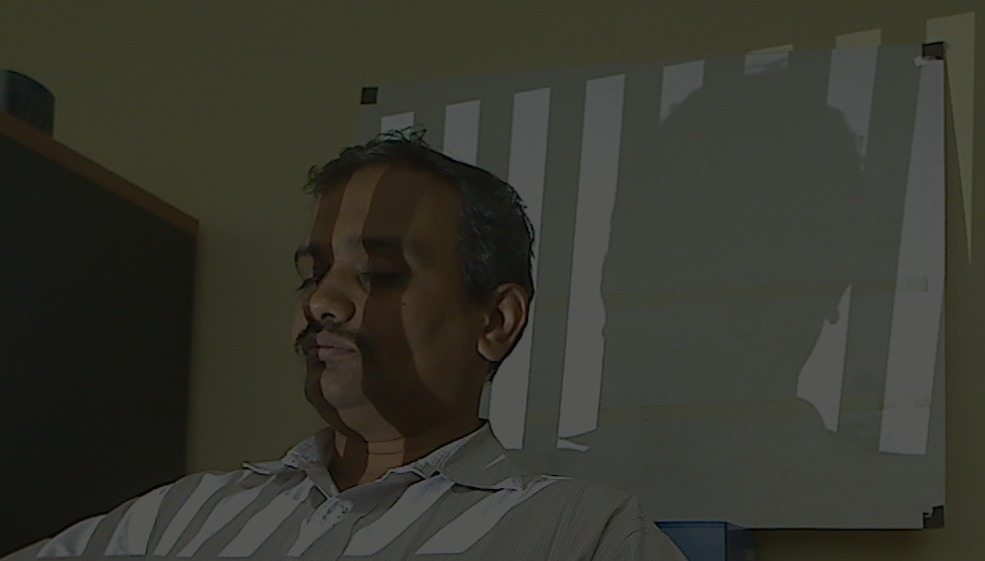
\includegraphics[width=3.5cm,height=3cm]{dependencies/img_source/cap_binary_v2.jpg}} &
\subfloat[]{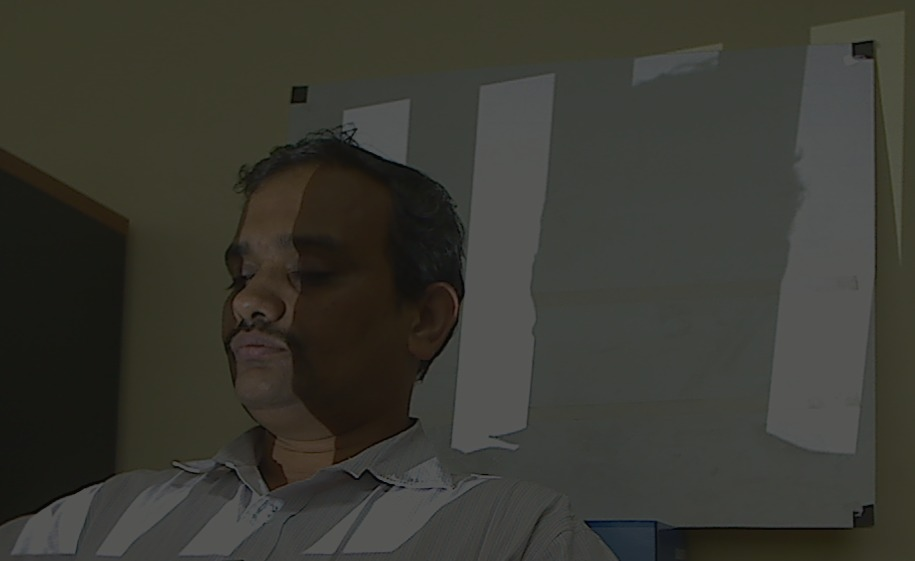
\includegraphics[width=3.5cm,height=3cm]{dependencies/img_source/cap_binary_v3.jpg}} \\
\end{tabular}
\end{tabularx}
\caption{Captured binary coded patterns}
\end{figure}
\end{frame}
%%%%%%%%%%%%%%%%%%%%%%%%%%%%%%%%%%%%%%%%%%%%%%%%%%%%%%%%%%%%%%%%%%%%%%%%%%%%%SLIDE ENDS%%%%%%%%%%%%%%%%%%%%%%%%%%%%%%%%%%%%%%%

%%%%%%%%%%%%%%%%%%%%%%%%%%%%%%%%%%%%%%%%%%%%%%%%%%%%%%%%%%%%%%%%%%%%%%%%%%%%%SLIDE starts%%%%%%%%%%%%%%%%%%%%%%%%%%%%%%%%%%%%%
\begin{frame}
\frametitle{Phase wrapping}
Assumed illumination model for 3 phase shifted pattern approach:
\begin{equation}
\begin{aligned}
& I_1^{v/h}=I_{dc}^{v/h}+I_{mod}^{v/h}*cos(\theta_{v/h}-\alpha) \\
& I_2^{v/h}=I_{dc}^{v/h}+I_{mod}^{v/h}*cos(\theta_{v/h}) \\
& I_3^{v/h}=I_{dc}^{v/h}+I_{mod}^{v/h}*cos(\theta_{v/h}+\alpha)
\end{aligned}
\end{equation}
Hence,
\begin{equation}
\begin{aligned}
& \theta_v=tan^{-1}\bigg[\frac{\sqrt[2]{3}(I_1^v-I_3^v)}{2I_2^v-I_1^v-I_3^v}\bigg],-\pi\leq\theta_v\leq\pi, \\
& \theta_h=tan^{-1}\bigg[\frac{\sqrt[2]{3}(I_1^h-I_3^h)}{2I_2^h-I_1^h-I_3^h}\bigg],-\pi\leq\theta_h\leq\pi 
\end{aligned}
\end{equation}

\begin{figure}[hb]
\begin{tabularx}{\linewidth}{@{}cXX@{}}
\begin{tabular}{c c}
\hspace{2cm}\subfloat[Vertical wrapped phase]{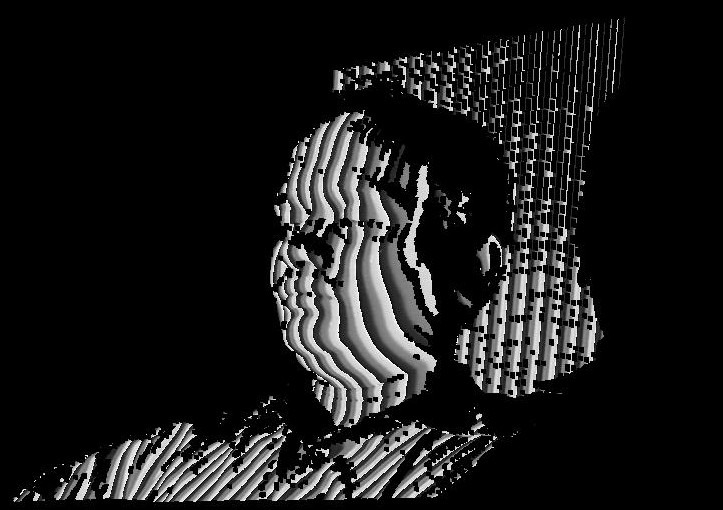
\includegraphics[width=3cm,height=3cm]{dependencies/img_source/wrapped_ver.jpg}} &
\hspace{1cm}\subfloat[Horizontal wrapped phase]{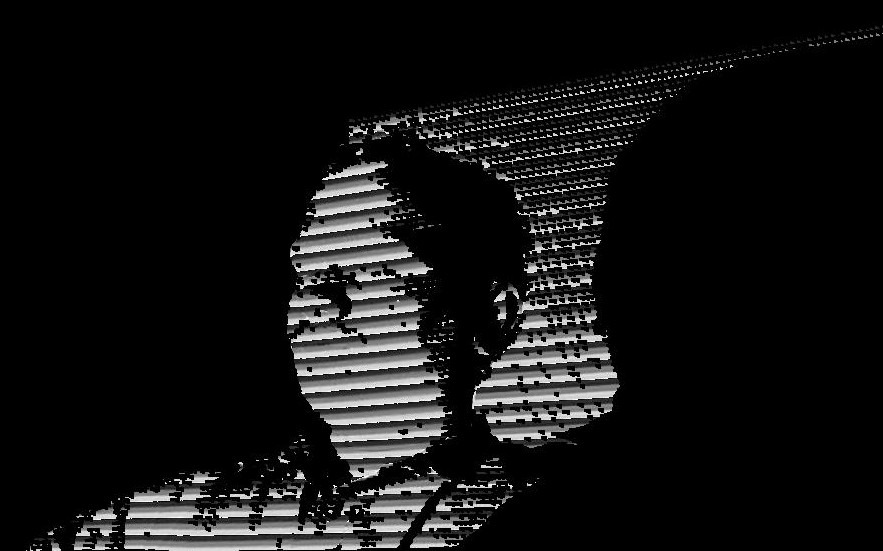
\includegraphics[width=3cm,height=3cm]{dependencies/img_source/wrapped_hor.jpg}}\\
\end{tabular}
\end{tabularx}
\caption{Computed wrapped phase}
\end{figure}
\end{frame}
%%%%%%%%%%%%%%%%%%%%%%%%%%%%%%%%%%%%%%%%%%%%%%%%%%%%%%%%%%%%%%%%%%%%%%%%%%%%%SLIDE ENDS%%%%%%%%%%%%%%%%%%%%%%%%%%%%%%%%%%%%%%%

%%%%%%%%%%%%%%%%%%%%%%%%%%%%%%%%%%%%%%%%%%%%%%%%%%%%%%%%%%%%%%%%%%%%%%%%%%%%%SLIDE starts%%%%%%%%%%%%%%%%%%%%%%%%%%%%%%%%%%%%%
\begin{frame}
\frametitle{Phase unwrapping module}
Unwrapped phase $(\psi_v,\psi_h)$ maps $(\theta_v,\theta_h)$ to its correct $2\pi$ multiple:
\begin{equation}
\begin{aligned}
& \psi_v=\theta_v+2\pi*C_v \\
& \psi_h=\theta_h+2\pi*C_h
\end{aligned}
\end{equation}
where,\newline
\indent 
$C_v(x,y)$: Decoded vertical binary code(or \textit{vertical period number}) at any pixel (x,y).\newline
$C_h(x,y)$: Decoded horizontal binary code(or \textit{horizontal period number}) at any pixel (x,y).
\begin{figure}[ht]
\begin{tabularx}{\linewidth}{@{}cXX@{}}
\begin{tabular}{l r}
\hspace{3cm}\subfloat[Vertical unwrapped phase]{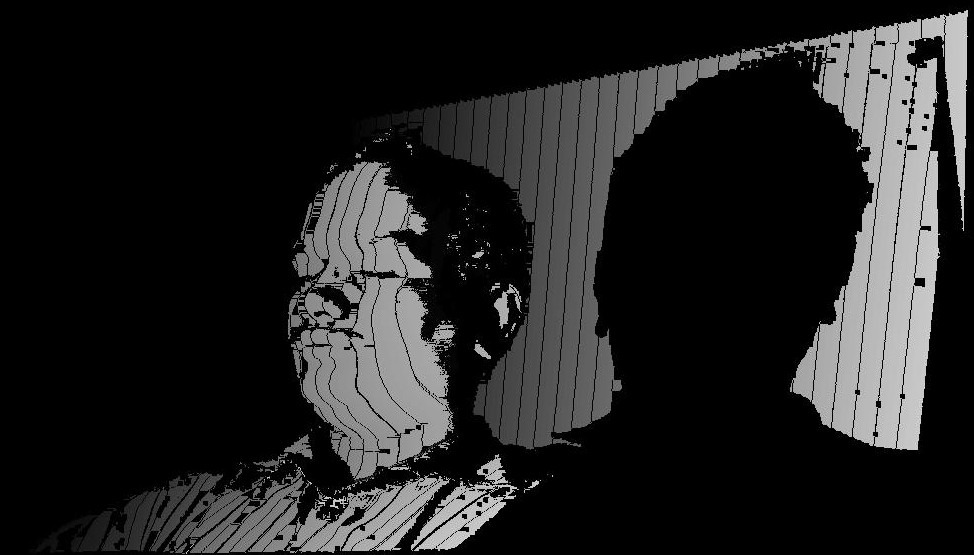
\includegraphics[width=3cm,height=3cm]{dependencies/img_source/unwrapped_ver.jpg}} &
\subfloat[Horizontal unwrapped phase]{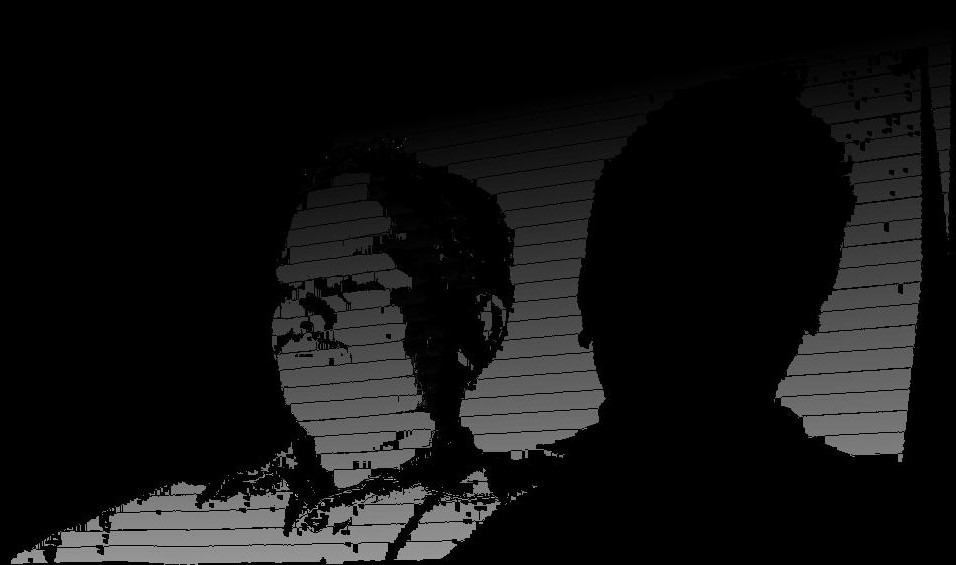
\includegraphics[width=3cm,height=3cm]{dependencies/img_source/unwrapped_hor.jpg}}\\
\end{tabular}
\end{tabularx}
\caption{Computed unwrapped phase}
\end{figure}
\end{frame}
%%%%%%%%%%%%%%%%%%%%%%%%%%%%%%%%%%%%%%%%%%%%%%%%%%%%%%%%%%%%%%%%%%%%%%%%%%%%%SLIDE ENDS%%%%%%%%%%%%%%%%%%%%%%%%%%%%%%%%%%%%%%%

%%%%%%%%%%%%%%%%%%%%%%%%%%%%%%%%%%%%%%%%%%%%%%%%%%%%%%%%%%%%%%%%%%%%%%%%%%%%%SLIDE starts%%%%%%%%%%%%%%%%%%%%%%%%%%%%%%%%%%%%%
\begin{frame}
\frametitle{Absolute phase computation}
Computing projector coordinates $(X_p,Y_p)$ corresponding to a camera coordinates $(X_c,Y_c)$
\begin{equation}
\begin{aligned}
& X_p=\lfloor w_{fringe}*\big(\frac{\psi_v}{2\pi}\big) \rfloor  ,
& Y_p=\lfloor w_{fringe}*\big(\frac{\psi_h}{2\pi}\big) \rfloor
\end{aligned}
\end{equation}
\begin{figure}
\begin{tabularx}{\linewidth}{@{}cXX@{}}
\begin{tabular}{c c}
\hspace{2cm}
\subfloat[Camera image]{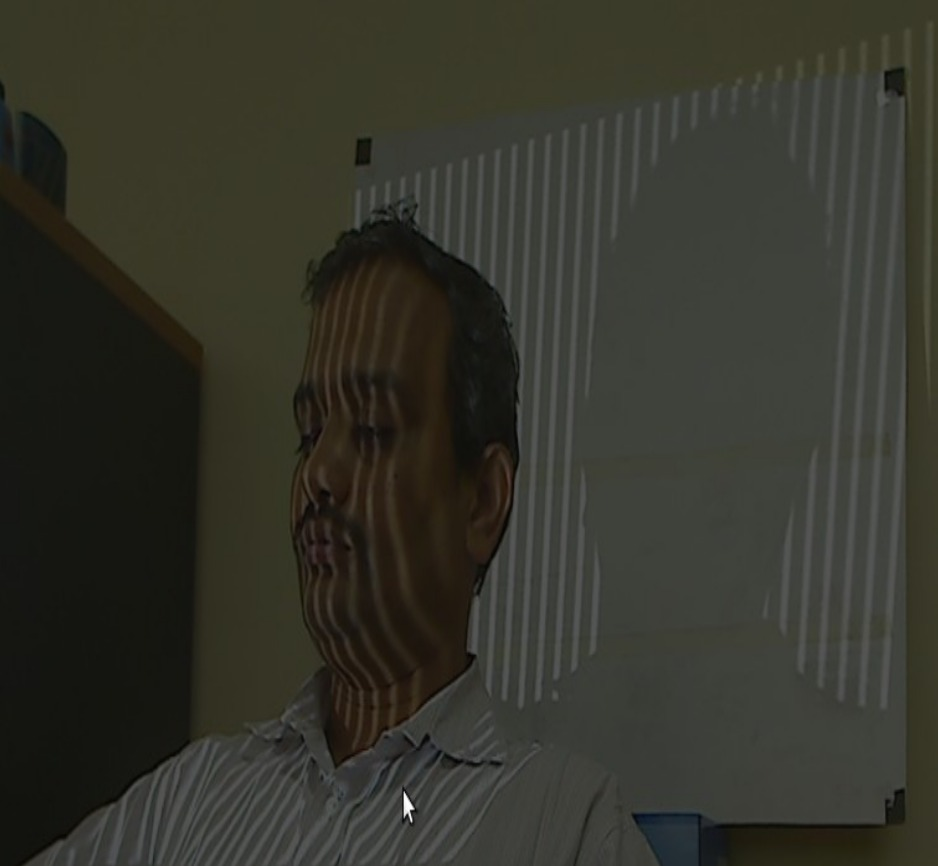
\includegraphics[width=3cm,height=3cm]{dependencies/img_source/camera_image.jpg}} &
\subfloat[Projector image]{
\includegraphics[width=3cm,height=3cm]{dependencies/img_source/projector_image.jpg}} 
\end{tabular}
\end{tabularx}
\caption{Stereo correspondence between camera and projector}
\end{figure}
\end{frame}
%%%%%%%%%%%%%%%%%%%%%%%%%%%%%%%%%%%%%%%%%%%%%%%%%%%%%%%%%%%%%%%%%%%%%%%%%%%%%SLIDE ENDS%%%%%%%%%%%%%%%%%%%%%%%%%%%%%%%%%%%%%%%

%%%%%%%%%%%%%%%%%%%%%%%%%%%%%%%%%%%%%%%%%%%%%%%%%%%%%%%%%%%%%%%%%%%%%%%%%%%%%SLIDE starts%%%%%%%%%%%%%%%%%%%%%%%%%%%%%%%%%%%%%
\begin{frame}
\frametitle{Triangulation}
\begin{figure}
\begin{tabularx}{\linewidth}{@{}cXX@{}}
\begin{tabular}{c c c c}
\hspace{-0.3cm}\subfloat[2D face image]{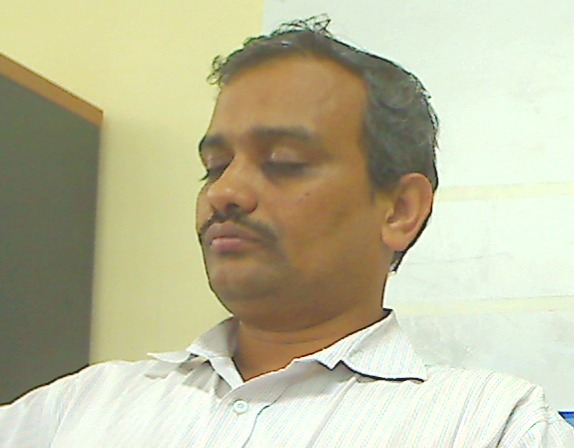
\includegraphics[width=3cm,height=3cm]{dependencies/img_source/face_2d.jpg}} & 
\hspace{-0.3cm}\subfloat[3D reconstruction of face]{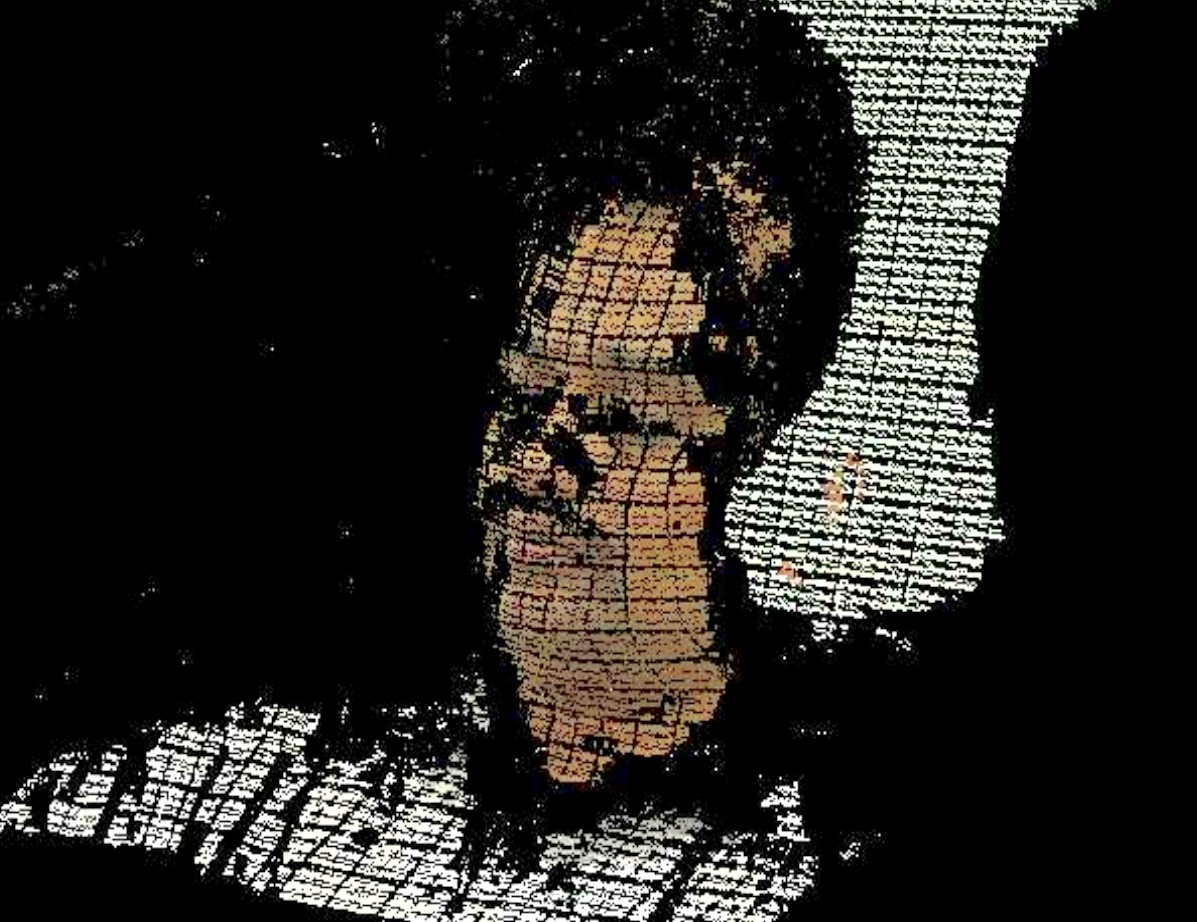
\includegraphics[width=3cm,height=3cm]{dependencies/img_source/face_3d.jpg}} &
\hspace{-0.3cm}\subfloat[2D image of box in front of wall]{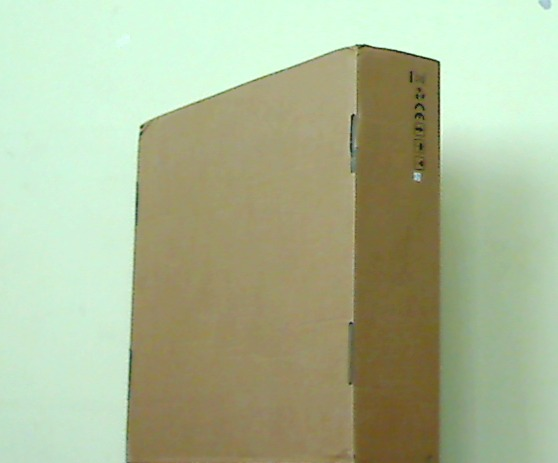
\includegraphics[width=3cm,height=3cm]{dependencies/img_source/box_wall_2d.jpg}} & 
\hspace{-0.3cm}\subfloat[3D reconstruction of box in front of wall]{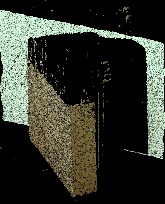
\includegraphics[width=3cm,height=3cm]{dependencies/img_source/box_wall_3d.jpg}}\\
\hspace{-0.3cm}\subfloat[2D image of a chair with background]{
\includegraphics[width=3cm,height=3cm]{dependencies/img_source/chair_2d.jpg}} &
\hspace{-0.3cm}\subfloat[3D reconstruction of chair with background]{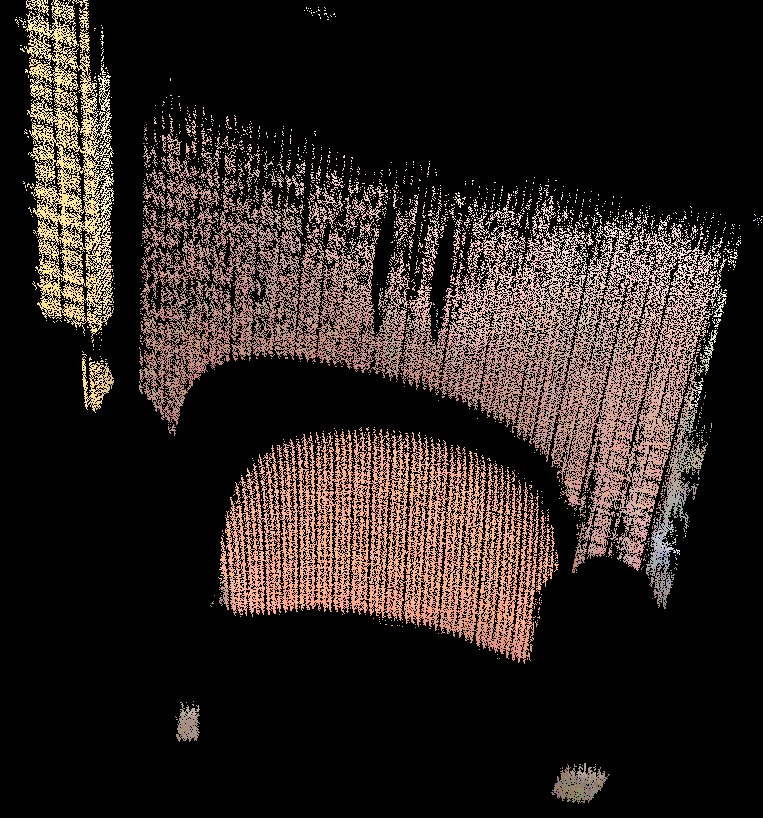
\includegraphics[width=3cm,height=3cm]{dependencies/img_source/chair_reconstruction.jpg}} &
\hspace{-0.3cm}\subfloat[A cup]{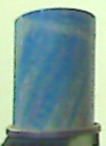
\includegraphics[width=3cm,height=3cm]{dependencies/img_source/cup_2d.jpg}} &
\hspace{-0.3cm}\subfloat[3D reconstruction of cup]{
\includegraphics[width=3cm,height=3cm]{dependencies/img_source/cup_3d.jpg}}\\ 
\end{tabular}
\end{tabularx}
\caption{Some 3D reconstruction results}
\end{figure}
\end{frame}
%%%%%%%%%%%%%%%%%%%%%%%%%%%%%%%%%%%%%%%%%%%%%%%%%%%%%%%%%%%%%%%%%%%%%%%%%%%%%SLIDE ENDS%%%%%%%%%%%%%%%%%%%%%%%%%%%%%%%%%%%%%%%

%%%%%%%%%%%%%%%%%%%%%%%%%%%%%%%%%%%%%%%%%%%%%%%%%%%%%%%%%%%%%%%%%%%%%%%%%%%%%SLIDE starts%%%%%%%%%%%%%%%%%%%%%%%%%%%%%%%%%%%%%
\begin{frame}
\frametitle{Accuracy evaluation}
We followed,
\begin{equation}
Accuracy=\frac{\sum_{p=1}^{vp}\Bigg[\frac{\sum_{i=1}^{vs_{p}}\Bigg[\bigg(\frac{|True_{p}-measured_{i}|}{True_{p}}\bigg)*100\Bigg]}{vs_{p}}\Bigg]}{vp}
\end{equation}
\begin{equation}
Precision=\frac{\sum_{p=1}^{vp}\Bigg[\frac{\sum_{i=1}^{vs_{p}}\Bigg[\bigg(\frac{|mean_{p}-measured_{i}|}{mean_{p}}\bigg)*100\Bigg]}{vs_{p}}\Bigg]}{vp}
\end{equation}
\begin{enumerate}
\item A checkerboard target was scanned 10 times at a distance of $\sim2.2$m from camera projector system. 
\item 6 individual lengths were measured using 3D data from scanner and compared against true values.
\item So, for our experiments we set $N$=10,vp=6.
\end{enumerate}
\end{frame}
%%%%%%%%%%%%%%%%%%%%%%%%%%%%%%%%%%%%%%%%%%%%%%%%%%%%%%%%%%%%%%%%%%%%%%%%%%%%%SLIDE ENDS%%%%%%%%%%%%%%%%%%%%%%%%%%%%%%%%%%%%%%%

%%%%%%%%%%%%%%%%%%%%%%%%%%%%%%%%%%%%%%%%%%%%%%%%%%%%%%%%%%%%%%%%%%%%%%%%%%%%%SLIDE starts%%%%%%%%%%%%%%%%%%%%%%%%%%%%%%%%%%%%%
\begin{frame}
\frametitle{Evaluation results}
\begin{figure}
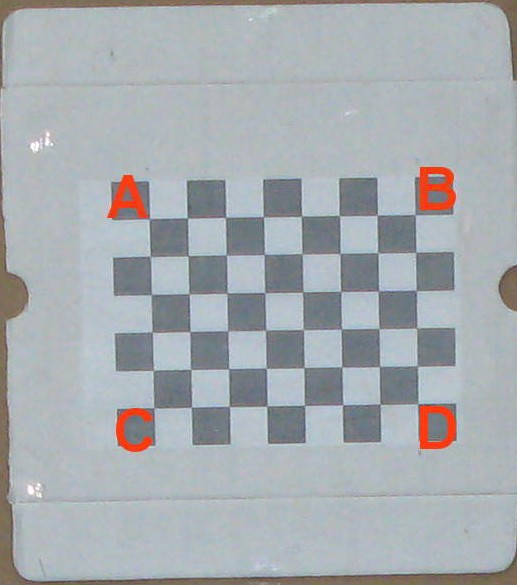
\includegraphics[width=3cm,height=3cm]{dependencies/img_source/measurement_object.jpg}
\caption{Measurement object}
\end{figure}
Length AB,BC,CD,AD,AC,BD were measured from 10 repetitions of 3D scans of object.
\begin{table}[!t]
\caption{Measurement accuracy and precision of
developed coded phase-shift 3D-scanner}
\centering
\begin{tabular}{|c| |c|}
\hline
Metric & Value(in \%)\\
\hline
Measurement accuracy & 0.61\\
Precision & 0.29 \\ 
\hline
\end{tabular}
\end{table}

\end{frame}
%%%%%%%%%%%%%%%%%%%%%%%%%%%%%%%%%%%%%%%%%%%%%%%%%%%%%%%%%%%%%%%%%%%%%%%%%%%%%SLIDE ENDS%%%%%%%%%%%%%%%%%%%%%%%%%%%%%%%%%%%%%%%

%%%%%%%%%%%%%%%%%%%%%%%%%%%%%%%%%%%%%%%%%%%%%%%%%%%%%%%%%%%%%%%%%%%%%%%%%%%%%SLIDE starts%%%%%%%%%%%%%%%%%%%%%%%%%%%%%%%%%%%%%
\begin{frame}
\frametitle{Conclusions}
\begin{enumerate}
\item Combination of binary coded and phase shift algorithm provides more 3D resolution than simple binary codes and higher noise resilience than phase shifted approach.     
\item Experimental system with measurement accuracy and precision within 1\% at distance of $\sim2.2$m from system.
 
\end{enumerate}
\end{frame}
%%%%%%%%%%%%%%%%%%%%%%%%%%%%%%%%%%%%%%%%%%%%%%%%%%%%%%%%%%%%%%%%%%%%%%%%%%%%%SLIDE ENDS%%%%%%%%%%%%%%%%%%%%%%%%%%%%%%%%%%%%%%%

%%%%%%%%%%%%%%%%%%%%%%%%%%%%%%%%%%%%%%%%%%%%%%%%%%%%%%%%%%%%%%%%%%%%%%%%%%%%%SLIDE starts%%%%%%%%%%%%%%%%%%%%%%%%%%%%%%%%%%%%%
\begin{frame}
Questions?
\end{frame}
%%%%%%%%%%%%%%%%%%%%%%%%%%%%%%%%%%%%%%%%%%%%%%%%%%%%%%%%%%%%%%%%%%%%%%%%%%%%%SLIDE ENDS%%%%%%%%%%%%%%%%%%%%%%%%%%%%%%%%%%%%%%%

\end{document}
